\documentclass[11pt,twoside,a4paper]{report}
\usepackage{a4}
\usepackage[ansinew]{inputenc}
\usepackage[danish]{babel}
\usepackage{textcomp}
\usepackage{paralist}		% for: \begin{compactitem}
\usepackage{subfigure}
\usepackage{paralist}		% for: \begin{compactitem}

\usepackage{graphicx}
\usepackage{fancyvrb} %centreret verbatim

\usepackage{listings, color}

\definecolor{forestgreen}{RGB}{34,139,34}
\definecolor{orangered}{RGB}{239,134,64}
\definecolor{darkblue}{rgb}{0.0,0.0,0.6}
\definecolor{gray}{rgb}{0.4,0.4,0.4}

\lstdefinestyle{XML} {
    language=XML,
    extendedchars=true, 
    breaklines=true,
    breakatwhitespace=true,
    emph={},
    emphstyle=\color{red},
    basicstyle=\ttfamily\small,
    columns=fullflexible,
    commentstyle=\color{gray}\upshape,
    morestring=[b]",
    morecomment=[s]{<?}{?>},
    morecomment=[s][\color{forestgreen}]{<!--}{-->},
    keywordstyle=\color{orangered},
    stringstyle=\ttfamily\color{black}, %\normalfont,
    tagstyle=\color{darkblue}\bf\normalfont,
    morekeywords={attribute,xmlns,version,type,release,name,xmlns:xsi,xmlns:xsd,minOccurs,maxOccurs,nillable,ref},
}


\lstdefinestyle{FAKE_XQUERY} {
    language=XML,
    alsolanguage=XSLT,
    extendedchars=true, 
    breaklines=true,
    breakatwhitespace=true,
    emph={},
    emphstyle=\color{red},
    basicstyle=\ttfamily\small,
    columns=fullflexible,
    commentstyle=\color{gray}\upshape,
    morestring=[b]",
    morecomment=[s]{<?}{?>},
    morecomment=[s][\color{forestgreen}]{<!--}{-->},
    keywordstyle=\color{orangered},
    stringstyle=\ttfamily\color{black}, %\normalfont,
    tagstyle=\color{darkblue}\bf\normalfont,
}


\lstdefinelanguage{XQUERY}
{
morekeywords={declare, namespace, function, attribute, string, as, dateTime, element, integer, node, not, where, if, than else,  for, in, return, current, text, data, name, doc, let, },
sensitive=false,
morestring=[b]",
moredelim=*[s][\color{darkblue}\bfseries]{\$}{\$}
}


\lstdefinestyle{SQL} {
    language=SQL,
    extendedchars=true, 
    breaklines=true,
    breakatwhitespace=true,
    emph={},
    emphstyle=\color{red},
    basicstyle=\ttfamily\small,
    columns=fullflexible,
    commentstyle=\color{gray}\upshape,
    morestring=[b]",
    morecomment=[s]{<?}{?>},
    morecomment=[s][\color{forestgreen}]{<!--}{-->},
    keywordstyle=\color{orangered},
    stringstyle=\ttfamily\color{black}, %\normalfont,
    tagstyle=\color{darkblue}\bf\normalfont,
    morekeywords={BEGIN, RETURN, FUNCTION, DECLARE, LANGUAGE},
}



\usepackage{fancyhdr}
\pagestyle{fancyplain} %til at lave overskrift p� hver side
%\setlength{\parindent}{0pt} %indrykning ved ny sektion
\fancyhf{} % delete current header and footer
\fancyhead[OL]{\leftmark}
\fancyhead[OR]{\thepage}
\fancyhead[EL]{\thepage}
\fancyhead[ER]{\leftmark} %giver overskrift \rightmark giver subsection overskrift
\fancypagestyle{plain}{%
\fancyhead{} % get rid of headers on plain pages
\renewcommand{\headrulewidth}{0pt} % and the line
}\pagestyle{fancy}
%ops�tning af TOC
\usepackage{hyperref} %make linkable
\hypersetup{
    colorlinks,
    citecolor=black,
    filecolor=black,
    linkcolor=black,
    urlcolor=black
}
\usepackage[toc,page]{appendix}

\setcounter{tocdepth}{2} %TOC only covers down to subsections
\setcounter{secnumdepth}{2} %section er det nederste niveau der tildeles nummer

\newcommand{\fct}[1]{\textit{#1}} %formatering for funktioner
\newcommand{\tbl}[1]{\textit{#1}} %formatering for tabeller
\newcommand{\flt}[1]{\emph{#1}} %formatering for felter
\newcommand{\ele}[1]{\emph{\textless #1\textgreater}} %formatering for felter
%\newcommand{\cmd}[1]{\textit{#1}} %formatering for entiteter
%\newcommand{\primkey}[1]{\underline{#1}} %formatering for primary key
%\newcommand{\schema}[1]{\emph{#1}} %formatering for skema

\title{Kompleks data og logik i databasen\\Brug af XML dokumenter til en videoapplikation}
\author{Stefan Jaensch, J�rgen Bo Arp Ladekj�r}
\date{Januar 2014 - Marts 2014}
\begin{document}
\maketitle
\newpage
\tableofcontents
\newpage

\chapter{Introduktion}
Videoapplikationer som Netflix, Youbio og Viaplay er blevet meget popul�re i de seneste par �r. Dette projekt handler om at skabe nogle de s�gefunktioner, som der m� v�re brug for i s�danne videoapplikationer, hvor et stort antal videoer er tilg�ngelige for brugeren. Disse s�gefunktioner skal g�re det muligt for brugeren at navigere rundt i de mange videoer og finde netop det indhold eller den specifikke video, som m�tte have interesse for brugeren.  

Som datakilde til dette projekt er der valgt et �bent API (Application Programming Interface) fra Danmarks Radio, som stiller stort set alt deres egenproducerede indhold tilg�ngeligt for brugeren/programm�ren via adressen http://www.dr.dk/nu/api . Dette API giver fx mulighed for at hente en total oversigt over alle tilg�ngelige videoer, i et enkelt XML dokument, samt hente p� detaljer omkring specifikke videoer.

I dette projekt hentes disse XML dokumenter ud via en standard webbrowser og gemmes lokalt, hvorefter de indl�ses i en BaseX XML database, hvorfra der vil bliver udarbejdet forskellige s�gefunktioner til foresp�rgsler i XML dokumenterne.

I �jeblikket findes der desv�rre ingen tilg�ngelig beskrivelse af struktur eller elementer i de tilg�ngelige XML dokumenter, s� derfor starter projektet med en analyse af netop strukturen eller elementerne i de XML dokumenter som er udvalgt til dette projekt.


\chapter{Unders�gelse af XML dokumenterne}\label{chapter:study-xml-documents}
I det �bne API fra Danmarks Radio er der mange forskellige XML dokumenter til r�dighed. Nogle af XML dokumenter er forholdsvis sm� og indeholder kun en sti til en grafik, som fx kan anvendes i en grafisk brugerflade. Til dette projekt er der udvalgt to store XML dokumenter, som indeholder beskrivelser af de enkelte videoer og den programserie som de evt. er en del af.

XML dokumenterne er hentet fra nedenst�ende adresser og deres struktur og indhold beskrives i underafsnittene her under.
\begin{itemize}
\item \textbf{http://www.dr.dk/nu/api/videos/all.xml}
\item \textbf{http://www.dr.dk/nu/api/programseries.xml}
\end{itemize}

\section{Beskrivelse af dokumentet all.xml}
Dette XML dokument indeholder information om alle videoer som er tilg�ngelige via API�et. Strukturen af dette dokument kan betragtes som v�rende relativ flad, da dybde i strukturen er relativ lille. Strukturen best�r udelukkende af rodelementet \ele{ArrayOfProgramSerieVideo}, som indeholder elementer af \ele{ProgramSerieVideo} for hver tilg�ngelig video der findes. Selve elementet \ele{ProgramSerieVideo} indeholder en r�kke elementer direkte under sig, som beskriver detaljerne omkring videoen. Disse detaljer er sidste niveau i strukturen, hvilket g�r at dybde af strukturen kan betragtes som v�rende flad. Skulle dybde �ges vil det fx v�re muligt ved at samle elementer som \ele{BitrateKbps}, \ele{Height} og \ele{Width} under et nyt element, fx med navnet \ele{TechDetails}. 

Omkring dokumentets indhold ses det at der er angivet en prolog, som fort�ller at dokumentet er XML version 1.0 og er skrevet med tegns�t UTF-8. Elementerne under elementet \ele{ProgramSerieVideo} er ikke beskrevet yderligere i API�et fra Danmarks Radio, s� de er i projektet fortolket p� f�lgende m�de:
\begin{itemize}
\item \textbf{Id:} Et unikt id for hver video der findes tilg�ngelig.
\item \textbf{Description:} En beskrivende tekst af hver video, som typisk anvendes i en tv-program-guide.
\item \textbf{ProgramSerieSlug:} Et navn som er tildelt videoer som er en del af en serie af programmer. Dette element kan betragtes som en slags fremmen�gle til elementet slug i XML dokumentet programseries.
\item \textbf{Title:} En beskrivende overskrift til videoen.
\item \textbf{Duration:} Videoen l�ngde (ikke set anvendt i endnu)
\item \textbf{BroadcastTime:} Tidspunkt for f�rst gang videoen blev vist i tv.
\item \textbf{ExpireTime:} Tidspunkt hvorefter videoen ikke vil v�re tilg�ngelig mere.
\item \textbf{PublishTime:} Tidspunkt hvor videoen blev gjort tilg�ngelig.
\item \textbf{Expired:} Er videoen ikke til tilg�ngelig mere?
\item \textbf{BroadcastChannel:} Tv-kanal som videoen blev sendt p�.
\item \textbf{VideoManifestUrl:} Link til streamning af videoen.
\item \textbf{VideoResourceUrl:} Link til streamning af videoen.
\item \textbf{Premiere:} Er denne video en premierevideo?
\item \textbf{BitrateKbps:} Datahastighed ved streamning af videoen. (Ikke altid sat)
\item \textbf{Height:} Videoens h�jdeopl�sning i pixels. (Ikke altid sat)
\item \textbf{Width:} Videoens bredeopl�sning i pixels. (Ikke altid sat)
\end{itemize}

\begin{figure}[ht]
%\centering
\begin{lstlisting}[style=XML]
<?xml version="1.0" encoding="utf-8"?>
<ArrayOfProgramSerieVideo 
 xmlns:xsi="http://www.w3.org/2001/XMLSchema-instance" 
 xmlns:xsd="http://www.w3.org/2001/XMLSchema">
  <ProgramSerieVideo>
    <Id>5062</Id>
    <Description>Det allerf�rste So ein Ding program ser p� HP Touch Smart IQ 500. Men hvor h�j er denne computers IQ egentlig?</Description>
    <ProgramSerieSlug>so-ein-ding</ProgramSerieSlug>
    <Title>Touch Smart sk�rme � So ein Ding</Title>
    <Duration />
    <BroadcastTime>2009-02-03T20:30:00</BroadcastTime>
    <ExpireTime>3000-01-01T00:00:00</ExpireTime>
    <PublishTime>0001-01-01T00:00:00</PublishTime>
    <Expired>false</Expired>
    <BroadcastChannel>DR2</BroadcastChannel>
    <VideoManifestUrl>http://www.dr.dk/Forms/Published/PlaylistGen.aspx?qid=1946138&amp;OnlyWritePath=True</VideoManifestUrl>
    <VideoResourceUrl>http://www.dr.dk/handlers/GetResource.ashx?id=853642</VideoResourceUrl>
    <Premiere>false</Premiere>
    <BitrateKbps>0</BitrateKbps>
    <Height>0</Height>
    <Width>0</Width>
  </ProgramSerieVideo>
  <!-- Herefter kommer mange flere ProgramSerieVideo elementer -->
</ArrayOfProgramSerieVideo>
\end{lstlisting}
\caption{Eksempel p� dokumentet all.xml}
\label{data:all.xml}
\end{figure}

\section{Beskrivelse af dokumentet programseries.xml}

Dette XML dokument indeholder information om alle serier af programmer, som er tilg�ngelige via API�et. Ved serier forst�s programmer som er opdelt i mange afsnit. Strukturen af dette dokument er lidt dybere end dokumentet all.xml, men ellers er den overordnet struktur identisk. Rodelementet hedder nu \ele{ArrayOfProgramSerie} og indeholder elementer af \ele{ProgramSerie}, som beskriver detaljer omkring selve serien af det specifikke program. Der hvor dokumentet adskiller sig dybdem�ssigt i forhold til dokumentet all.xml er i elementet \ele{Labels} som kan indeholde en til mange elementer med navnet \ele{String}, som er en kategorisering af seriens emne.

I dokumentets indhold ses en prolog, som er identisk for det forrige dokuments prolog. Igen er elementerne under elementet \ele{ProgramSerie} ikke beskrevet yderligere i API�et fra Danmarks Radio, s� de er i projektet fortolket p� f�lgende m�de:

\begin{itemize}
\item \textbf{Slug:} Unik n�gle et den enkelte serie af programmer. Denne n�gle anvendes som en slags fremmen�gle i det forrige dokument (all.xml).
\item \textbf{Title:} En beskrivende overskrift til serien af programmet.
\item \textbf{Description:} En beskrivende tekst af hver serie, som typisk anvendes i en tv-program-guide.
\item \textbf{ShortName:} (Ikke set anvendt)
\item \textbf{NewestVideoId:} En slags fremmen�gle til id�et p� den nyeste video i dokumentet all.xml.
\item \textbf{NewestVideoPublishTime:} Tidspunkt for udgivelse af den nyeste video i serien af programmet.
\item \textbf{VideoCount:} Antal af videoer i denne serie af programmer.
\item \textbf{Labels:} Kategorisering af series indhold.
\item \textbf{String:} En kort beskrivende tekst til kategorisering under Labels.
\end{itemize}  

\begin{figure}[ht]
%\centering
\begin{lstlisting}[style=XML]
<?xml version="1.0" encoding="utf-8"?>
<ArrayOfProgramSerie 
 xmlns:xsi="http://www.w3.org/2001/XMLSchema-instance" 
 xmlns:xsd="http://www.w3.org/2001/XMLSchema">
  <ProgramSerie>
    <Slug>so-ein-ding</Slug>
    <Title>So ein Ding</Title>
    <Description>Det bliver ikke nemmere. Den allersidste Ding er ...</Description>
    <ShortName />
    <NewestVideoId>96149</NewestVideoId>
    <NewestVideoPublishTime>2014-01-09T11:39:28</NewestVideoPublishTime>
    <VideoCount>157</VideoCount>
    <Labels>
      <string>tech og viden</string>
    </Labels>
    <WebCmsImagePath />
  </ProgramSerie>
  <!-- Herefter kommer mange flere ProgramSerie elementer -->
</ArrayOfProgramSerie>
\end{lstlisting}
\caption{Eksempel p� dokumentet programseries.xml}
\label{data:programseries.xml}
\end{figure}







\chapter{Validering af XML dokumenterne}\label{chapter:xml-schemas}
Som beskrevet i det foreg�ende kapitel, s� er der ikke i API'et ikke udstillet noget validerings-skema eller nogen indbygget DTD (Document Type Definition) til de XML dokumenter der er til r�dighed. Den manglende mulighed for at validere XML dokumenterne betyder, at videoapplikation m� stole p� at XML dokumenterne altid overholder samme struktur. �ndres strukturen pludseligt vil det betyde at de s�gefunktioner, som udarbejdes i dette projekt, ikke vil kunne fungere l�ngere. Det er dermed sagt, at der kun gives garanti for at alle de funktioner, som udarbejdes i dette projekt kun kan anvendes s�fremt at de XML dokumenter, som hentes fra Danmarks Radio's API, kan valideres imod de XML skemaer, som beskrives i dette kapitel. 

Nogle af fordelene ved at anvende XML skema fremfor DTD er, at XML skema er meget mere kraftfuldt end DTD da XML skema eksempelvis underst�tter datatyper og desuden er selve XML skemaer selv beskrevet med XML Syntax og derfor er relative lette at l�se.

\section{Beskrivelse af XML skemaerne}
Ved unders�gelse af XML dokumenterne fremgik det at begge XML dokumenter indeholder en sekvens af enten videoer eller programserier. Derfor best�r f�rste del af begge de udarbejde XML skemaer af en sekvens af enten elementet ProgramSerieVideo eller elementet ProgramSerie, som kan forekomme uendeligt mange gange. B�de elementet ProgramSerieVideo og ProgramSerie er oprettet som et complexType element, der best�r af hver sine beskrivende elementer, som fx Slug, Title, Description osv. Disse elementer som beskriver videoen eller programserien er blevet sat til at v�re af en bestemt type. Valget af type til elementerne er fremkommet dels af elements navn og elements indhold, som har givet et hint om hvilke type der er tale om.

Specielt skal det bem�rkes at elementet \ele{BroadcastTime} i �ProgramSerieVideo� er sat til at kunne forekommer i XML dokumentet med en null v�rdi (nillable). Det vil sige at en enkelt video kan have elementet � BroadcastTime � i sig, men uden nogen v�rdi. En anden speciel detalje er at elementet BroadcastChannel i �ProgramSerieVideo�, er sat til at kunne undlades helt i en video. Dette g�lder �vrigt ogs� ShortName, WebCmsImagePath i skemaet til ProgramSeries.

I skemaet til ProgramSeries er det ogs� v�rd at bem�rke element LabelsType, som er et complexType element, som indg�r i et andet complexType element, nemlig elementet ProgramSerieType.  

\begin{figure}[ht]
%\centering
\begin{lstlisting}[style=XML]
<?xml version="1.0"?>
<xs:schema xmlns:xs="http://www.w3.org/2001/XMLSchema">
	<xs:element name="ArrayOfProgramSerieVideo">
		<xs:complexType>
			<xs:sequence>
				<xs:element name="ProgramSerieVideo" 
				            maxOccurs="unbounded"
							type="ProgramSerieVideoType" />
			</xs:sequence>
		</xs:complexType>
	</xs:element>	
	<xs:complexType name="ProgramSerieVideoType">
		<xs:sequence>
			<xs:element name="Id" 					
				        type="xs:nonNegativeInteger" />
			<xs:element name="Description" 			
				        type="xs:string" />
			<xs:element name="ProgramSerieSlug" 	
				        type="xs:string" />
			<xs:element name="Title" 				
				        type="xs:string" />
			<xs:element name="Duration" 			
				        type="xs:string" />
			<xs:element name="BroadcastTime" 		
				        type="xs:dateTime" 
						nillable="true" />
			<xs:element name="ExpireTime" 			
				        type="xs:dateTime" />
			<xs:element name="PublishTime" 			
				        type="xs:dateTime" />
			<xs:element name="Expired" 				
				        type="xs:boolean" />
			<xs:element name="BroadcastChannel" 	
				        type="xs:string" 
						minOccurs="0" 
						maxOccurs="1" />
			<xs:element name="VideoManifestUrl" 	
				        type="xs:anyURI" />
			<xs:element name="VideoResourceUrl" 	
				        type="xs:anyURI" />
			<xs:element name="Premiere" 			
				        type="xs:boolean" />
			<xs:element name="BitrateKbps" 			
				        type="xs:nonNegativeInteger" />
			<xs:element name="Height" 				
				        type="xs:nonNegativeInteger" />
			<xs:element name="Width" 				
				        type="xs:nonNegativeInteger" />
		</xs:sequence>
	</xs:complexType>
</xs:schema>
\end{lstlisting}
\caption{XML skema til dokumentet all.xml}
\label{data:all_schema.xsd}
\end{figure}


\begin{figure}[ht]
%\centering
\begin{lstlisting}[style=XML]
<?xml version="1.0"?>
<xs:schema xmlns:xs="http://www.w3.org/2001/XMLSchema">
	<xs:element name="ArrayOfProgramSerie">
		<xs:complexType>
			<xs:sequence>
				<xs:element name="ProgramSerie" maxOccurs="unbounded" type="ProgramSerieType"/>
			</xs:sequence>
		</xs:complexType>
	</xs:element>
	<xs:complexType name="ProgramSerieType">
		<xs:sequence>
			<xs:element name="Slug" 			type="xs:string" />
			<xs:element name="Title" 			type="xs:string" />
			<xs:element name="Description" 		type="xs:string" />
			<xs:element name="ShortName" 		type="xs:string" minOccurs="0" maxOccurs="1" />
			<xs:element name="NewestVideoId"	type="xs:nonNegativeInteger" />
			<xs:element name="NewestVideoPublishTime" type="xs:dateTime" />
			<xs:element name="VideoCount"		type="xs:nonNegativeInteger" />
			<xs:element name="Labels"			type="LabelsType" />
			<xs:element name="WebCmsImagePath" type="xs:anyURI" minOccurs="0" maxOccurs="1" />
		</xs:sequence>
	</xs:complexType>
	<xs:complexType name="LabelsType">
		<xs:sequence>		
			<xs:element name="string"	type="xs:string" minOccurs="0" maxOccurs="unbounded" />
		</xs:sequence>	
	</xs:complexType>	
</xs:schema>
\end{lstlisting}
\caption{XML skema til dokumentet programseries.xml}
\label{data:programseries.xsd}
\end{figure}

\section{Validering med XML skema}

Valideringen af XML dokumenterne med XML skemaerne er test ved hj�lp af BaseX, hvor validate:xsd er blevet anvendt. For at test XML skemaerne holder over tid, s� er der igennem projektetsforl�b blevet hentet nye versioner af XML dokumenterne, s� ogs� har best�et valideringstesten med de udarbejde XML skemaer. 

\begin{figure}[ht]
%\centering
\begin{lstlisting}[style=FAKE_XQUERY, language=XQUERY]
validate:xsd('all.xml', 'all_schema.xsd')
\end{lstlisting}
\caption{Funktionskald til validering af all.xml med skemaet all\_schema.xsd}
\label{xschema: validering }
\end{figure}


\chapter{XQuery og XPath s�gning}\label{chapter:xquery-search}

\section{Find alle kategorierne til programserierne}
Brugeren af videoapplikationen skal have muligheden for at navigere imellem de forskellige programserieres kategorier, som der findes p� et givent tidspunkt. Funktionen i figur \ref{xquerySearch:getProgramSeriesCategory} bruger et XPath udryk til at finde alle kategori navnene i XML dokumentet og funktionen distinct-value() selekterer kun unik navne. En �for lykke� returnerer kategorinavne som et element, \ele{category}, og derudover returnerer funktionen getProgramSeriesCategory() et element, \ele{countCategory}, med antal af forskellige kategorier. 

\begin{figure}[ht]
%\centering
\begin{lstlisting}[style=FAKE_XQUERY, language=XQUERY]

declare function dr:getProgramSeriesCategory
  ( $programseriesFileName as xs:string) as element()*{
    
    let $progSerieLabels := distinct-values(doc($programseriesFileName)/ArrayOfProgramSerie/ProgramSerie/Labels/
    	string/text())
    return (
      <countCategory>{count($progSerieLabels)}</countCategory>,
      (
      for $label in $progSerieLabels
        return <category>{$label}</category>
      )
    )
};

\end{lstlisting}
\caption{Funktion til at finde kategorinavne og samlet antal af kategorier.}
\label{xquerySearch:getProgramSeriesCategory}
\end{figure}


\section{Find antal programserier i en kategori}
N�r en bruger v�lger en kategori skal videoapplikationen vise antallet af programserier i kategorien og forskellige informationer om disse. I funktionen \ref{xquerySearch:programSeriesOfCategory} finder XPath udtrykket alle \ele{ProgramSerie} elementer, hvor elementet \ele{string} i elementet \ele{Labels} har den sammen v�rdi som den valgte kategori. Variablen \$progSeries indeholder en sekvens med alle fundende \ele{ProgramSerie} elementer og ikke kun elementet \ele{Labels} fordi /.. ved slutning af sekvensen v�lger for�ldre elementet, som er \ele{ProgramSerie}.  XQuery funktionen count() t�ller antallet af fundende \ele{ProgramSerie} elementer. Denne information og alle de fundende \ele{ProgramSerie} elementer bliver returneret i elementet \ele{programSeriesCategory}.

\begin{figure}[ht]
%\centering
\begin{lstlisting}[style=FAKE_XQUERY, language=XQUERY]

declare function dr:programSeriesOfCategory
  ( $programseriesFileName as xs:string, $category as xs:string ) as element()*{
    
    let $progSeries := doc($programseriesFileName)/ArrayOfProgramSerie/
    ProgramSerie/Labels[string=$category]/..
    return (
      <programSeriesCategory>
        <nameCategory>{$category}</nameCategory>
        <countProgSeries>{count($progSeries)}</countProgSeries>
        {
         for $progSerie in $progSeries
           return $progSerie
         }
      </programSeriesCategory>
    )
};

\end{lstlisting}
\caption{Funktion til at finde antallet af programserier i en bestemt kategori.}
\label{xquerySearch:programSeriesOfCategory}
\end{figure}

\section{Find nyeste videoer inden for en specifik kategori}

For at videoapplikationen kan pr�sentere detaljeret videoinformationer og de nyeste videoer, n�r en bruger har valgt en kategori, er det n�dvendigt at hente information fra XML dokumentet all.xml. Informationerne om de enkelte videoer ligger alts� ikke i det sammen XML dokument, hvor informationen om programserierne og kategorier er gemt. I dette tilf�lde findes kategori informationer i dokumentet programseries.xml og videoinformationen i dokumentet all.xml. Et unikt video- ID som hedder \ele{NewestVideoId} i dokumentet programseries.xml og \ele{Id} i dokumentet all.xml referere fra et specifikt \ele{programserie} element til et specifikt \ele{ProgramSerieVideo} element. Her vises sig en svaghed ved XML som ikke har nogle begr�nsninger p� dataindholdet (fx unik) og fremmen�gle referencer mellem elementerne. Faktisk er der ingen information i de to XML dokumenter eller deres XML skemaer, som dokumenterer denne reference imellem elementerne i de to dokumenter.
Til s�gning efter alle programserier i en specifik kategori eksisterer der allerede en funktion som hedder programSeriesOfCategory() som er vist i figur \ref{xquerySearch:programSeriesOfCategory}. Denne funktion blev kaldt i funktionen videosOfCategory() i figur \ref{xquerySearch:videosOfCategory}. Den resulterende sekvens indeholder alle fundende \ele{programserie} elementer, som igen har det s�gte tag \ele{NewestVideoId}. En �for lykke� behandler elementerne \ele{programserie} og et XPath udtryk selekterer kun det unik video ID, som blev gemt i variabelen \$videoId. I den samme �for lykke� bliver \$videoId brugt som et argument i en anden XPath s�gning, men denne gang i videodokumentet  all.xml. Resultatet af funktionens s�gningen er elemeter af \ele{programSerieVideo} med tilh�rende detaljeret informationer.


\begin{figure}[ht]
%\centering
\begin{lstlisting}[style=FAKE_XQUERY, language=XQUERY]

declare function dr:videosOfCategory
( $programseriesFileName as xs:string,  $programseriesVideoFileName as xs:string, $category as xs:string ) as element()*{

  let $programSeriesCategory := dr:programSeriesOfCategory($programseriesFileName, $category )
  return(
    for $videoId in $programSeriesCategory//ProgramSerie/NewestVideoId/data()
      return(
        let $programSerieVideo := doc($programseriesVideoFileName)//ProgramSerieVideo[Id = $videoId]
        return $programSerieVideo
      )
  )
};
\end{lstlisting}
\caption{Funktion til at finde nyeste videoer inden for en specifik kategori.}
\label{xquerySearch:videosOfCategory}
\end{figure}




\section{Find alle videoer inden for et specifikt tidsinterval}

Videoapplikationen skal have en s�gefunktion, hvor brugeren kan finde alle de programserievideoer, hvor udsendelsestidspunktet ligger inden for et specifikt tidsinterval. XQuery funktionen er vist i figur \ref{xquerySearch:programSeriesVideoBroadcastDateInterval} og tager imod navnet af XML videofilen, start og stop tidspunktet, som argumenter til funktionen. En �for lykke� l�ser tidsinformation i tagget \ele{BroadcastTime} af hvert element \ele{ProgramSerieVideo} og returnerer kun de \ele{ProgramSerieVideo} elementer, hvor udsendelsestidspunktet ligger inden for tidsintervallet. XQuery har to forskellige sammenligningsoperatorer, v�rdier sammenligningsoperatorer fx (le, ge) som er beregnet til at sammenligne enkelte v�rdier og generelle sammenligningsoperatorer fx (\textless=, =\textgreater) for at sammenligne sekvenser med flere v�rdier. I denne funktion blev der brugt den f�rste variant fordi det kun er enkelte v�rdier som skal sammenlignes. Det er n�dvendig at tage h�jde for at tagget \ele{BroadcastTime} kan v�re tomt. I denne situation vil cast fra null til xs:dateTime() giver en dynamisk fejl. XQuery er et funktionelt programmeringssprog og der medf�lges at variabler er uforanderlige. Derfor bruges en hj�lpefunktion, figur \ref{xquerySearch:getBroadCastTime} som kontrollerer om tagget er tomt og dermed returnere en dummy dato ("1900-01-01T00:00:00") ellers den fundende dato, til at opdatere den interne variabel \$broadCastTime.

\begin{figure}[ht]
%\centering
\begin{lstlisting}[style=FAKE_XQUERY, language=XQUERY]

declare function dr:programSeriesVideoBroadcastDateInterval
( $programseriesVideoFileName as xs:string, $dateStart as xs:dateTime, $dateStop as xs:dateTime) as element()*{
  for $progSerVideoElement in doc($programseriesVideoFileName)/ArrayOfProgramSerieVideo/ProgramSerieVideo
  let $broadCastTime := dr:getBroadCastTime($progSerVideoElement/BroadcastTime)
  where $broadCastTime ge $dateStart and $broadCastTime le $dateStop
  return $progSerVideoElement
}; 

\end{lstlisting}
\caption{Funktion til at finde videoer for et specifikt tidsinterval}
\label{xquerySearch:programSeriesVideoBroadcastDateInterval}
\end{figure}



\begin{figure}[ht]
%\centering
\begin{lstlisting}[style=FAKE_XQUERY, language=XQUERY]

declare function dr:getBroadCastTime
($broadCastTimeElement as element() ) as xs:dateTime{
  if( not($broadCastTimeElement/data()) ) then (
       (xs:dateTime("1900-01-01T00:00:00"))
    ) else (
      (xs:dateTime($broadCastTimeElement/data()))
    ) 
};

\end{lstlisting}
\caption{Funktion til at l�se BroadcastTime}
\label{xquerySearch:getBroadCastTime}
\end{figure}





%TODO: Insert stuff about xquery search

% Description of each search and how it is solved

% Done! Find programs between specific date intervals.
% Done! Find all kinds of labels for prorgams.
% Done! Find the number of programs for each label.

% Identisk! Find all kinds of broadcasting channels.
% Find the number of programs for each channel.

% Find all videos from a particular series of programs sorted by date.





\chapter{Fuld tekst s�gning}\label{chapter:full-text-search}
I videoapplikation vil der v�re behov for at kunne s�ge efter videoer eller programserier ud fra specifikke ord, som kan v�re en del af titlen eller fx beskrivelsen, som er den del der indeholder mest tekst.  

\section{Oprettelse af full-text index}

I BaseX databasen er det muligt at oprette et "full-text index" til sin XML database. Index�et vil bliver oprettet p� indhold af alle elementer i XML dokumentet og ikke kun p� et specifikt element i dokumentet. Sammenlignes dette med en relationel database vil det svare til, at index�et ikke kun oprettes p� en specifik kolonne i en specifik tabel, men p� data i alle kolonner i alle tabeller i databasen. 

\subsection{Indstillinger til full-text index}

Ved oprettelsen af index�et skal sproget angives, ellers s�ttes det default til engelsk. I denne videoapplikation vil sproget v�re dansk og det f�r stor betydning n�r teksterne i databasen uds�ttes for �Stemming�. Stemming er en proces, som reducere ord ned til deres mindste form. Det vil fx sige at et ord som �Bilerne� vil blive til �bil�, f�r det gemmes som en v�rdi i index�et. Der kan ogs� tilf�jes en "stop word list", som er en liste af ord, der ikke �nskes medtaget i index'et.  

\section{Full-text s�gning}

Det skal i videoapplikationen v�re muligt at s�ge efter specifikke ord inden for en specifik kategori af programserier. Det vil sige at full-text s�gningen skal kombineres med en XQuery-foresp�rgelse, hvor kun elementer, som indg�r i den efterspurgte kategori af programserier medtages og kun returneres som resultat, hvis de ogs� kan opfylde full-text s�gningen. 
Denne s�gning ses i figur \ref{fulltextSearch:programserierLivsstilOrd}.

\begin{figure}[ht]
%\centering
\begin{lstlisting}[style=FAKE_XQUERY, language=XQUERY]
//ArrayOfProgramSerie/ProgramSerie/Labels[string='livsstil']/..
         /Description[ft:contains(text(), ("restaurant", "laks"), { "mode": "any" })]/..
\end{lstlisting}
\caption{Implementationen af s�gning efter specifik kategori af programserier med specifikke ord som indhold.}
\label{fulltextSearch:programserierLivsstilOrd}
\end{figure}

\section{En sky af ord}

Til videoapplikationen �nskes et flot baggrundsbillede, som best�r af en sky af de mest brugte ord i alle elementerne, som beskriver programserierne. Til at skabe s�dan et billede skal full-text index�et unders�ges. 
Indholdet skal tages ud i en r�kkef�lge, hvor de mest brugte ord kommer f�rst og hvor der med hvert ord f�lger et tal, som beskriver hvor mange gange ordet er anvendt.
I figur \ref{fulltext:beforeStopWords} ses et eksempel p�, hvordan det kommer til at se ud n�r der dannes et billede af ordene i index'et. 
Billedet i figuren illustrere dog ogs� et lille problem, da ordene er simple ord som "og", "der", "at" osv. Dette l�ses ved at indf�re en "stop word list".

\begin{figure}[ht]
  \centering
   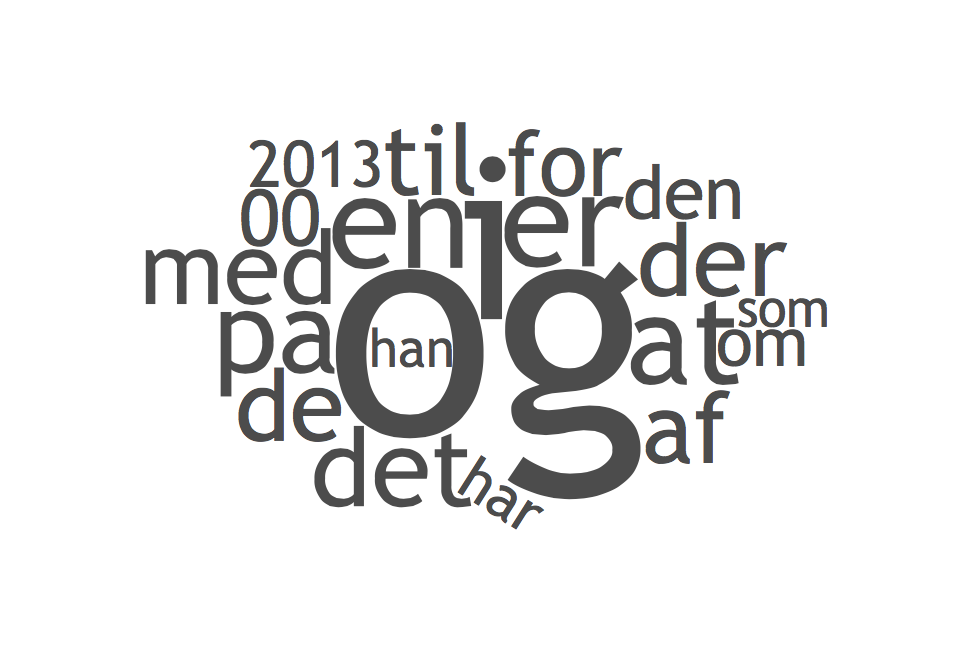
\includegraphics[width=1.1\textwidth]{pic/wordcloud1b.png}
   \caption{Eksempel p� billede f�r indf�relse af "stop word list".}
   \label{fulltext:beforeStopWords}
\end{figure}

\subsection{Tilf�jelse af stop word list}

Da ikke alle ord er lige interesant, at have med i index�et, s� er det muligt at oprette en "stop word list", som indeholder alle de ord, som skal undtages n�r et full-text index�et oprettes. 
I dette projekt er denne "stop word list" blevet oprettet ved at unders�ge de meste brugte ord i index'et uden "stop word list" og derefter tilf�je dem til listen, som ikke giver mening i et full-text index.
I figur \ref{fulltext:afterStopWords} ses nu hvordan udvalget af ord er blevet bedre.

\begin{figure}[ht]
  \centering
   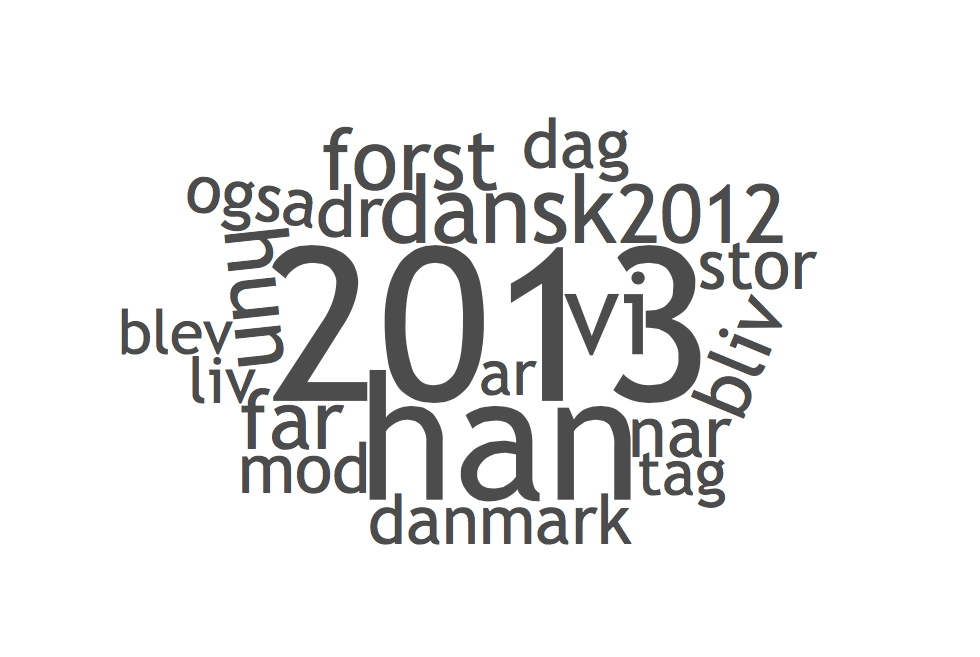
\includegraphics[width=1.1\textwidth]{pic/wordcloud2c.png}
   \caption{Eksempel p� billede efter indf�relse af "stop word list".}
   \label{fulltext:afterStopWords}
\end{figure}

\chapter{Join imellem XML dokumenter}\label{chapter:joining-data}
I dette kapitel beskrives forskellige funktioner, som alle har det tilf�ldes at de alle arbejder p� 2 forskellige XML dokumenter samtidigt eller 2 versioner af samme XML dokumenter, men af forskellige dato. 

\section{Antal tilg�ngelige afsnit i en programserie}
Det er ikke altid at alle afsnit af et specifikt program er tilg�ngeligt i en programserie. Eksempelvis vil Danmarks Radio kun have et begr�nset antal af afsnit, liggende tilg�ngeligt for brugerne, n�r det drejer sig om relativt kostbarer produktioner som dramaserier, der efterf�lgende skal kunne s�lges p� eksempelvis DVD. I disse tilf�lde vil eksempelvis kun de 2 sidste afsnit v�re tilg�ngelige i en kort periode.

Det er derfor interessant at f� udarbejdet en funktion, som kan returnere det totale antal af afsnit samt antallet af afsnit som er tilg�ngelige netop nu.

Til dette form�l skal elementet med navnet VideoCount, fra dokumentet programseries.xml, anvendes som det antal af afsnit, der total findes i en specifik programserie. Til at finde antallet af afsnit, som faktisk er tilg�ngelige netop nu, bruges aggregeringsfunktionen Count p� elementerne med navnet ProgramSerieVideo i dokumentet all.xml, hvor det angives som betingelse, at der kun skal medtage de elementer, som indeholder samme v�rdi i elementet ProgramSerieSlug som i elementet Slug fra dokumentet programseries.xml.  Desuden �nskes kun de videoer, som har elementet Expired sat til falsk, da det kunne t�nkes at en video ikke er blevet fjernet fra dokumentet all.xml, men at selve linket til videoen ikke er gyldig l�ngere. 

For at skabe et resultatset, for en helt specifik programserie (Slug), som kun indeholder antal videoer total og antal tilg�ngelige videoer, for en helt specifike programserie, s� er der implementeret 2 funktioner, som hedder henholdsvis checkVideoCount og countVideoSlugs.

Funktionen checkVideoCount tager imod 3 argumenter, som alle er af datatype string. SlugName er navnet p� selve programserien fx �so-ein-ding�, de 2 �vrige argumenter er navnene p� XML filerne, som henholdsvis indeholder listen af programserier (programseriesFileName) og liste over alle de enkelte videoer (videoFileName). Funktionen starter med at bruge et XPath-udtryk til at finde f�rste del af resultats�ttet, som er indholdet af elementet VideoCount, fra listen af programserier. Derefter kaldes en hj�lpefunktion, som hedder countVideoSlugs, hvor aggregeringsfunktionen count anvendes til samment�lle antallet af afsnit, som findes i XML dokumentet, der indeholder alle videoer. Betingelse for at blive talt med er, som tidligere n�vnt, at elementet Expired skal v�re sat til v�rdien falsk. Hj�lpefunktionen sender resultatet retur som en integer til funktionen checkVideoCount. Det samlede resultatset returens nu som en sekvens best�ende af to elementer: totalVideoCount og availableVideoCount. For at kunne returnere en sekvens af elementer, er funktionen checkVideoCount defineret til at returnere element()* som betyder at 0 til mange elementer kan forventes returneret fra funktionen. I dette tilf�lde vil antallet af elementer dog altid v�re 2, hvoraf det ene element (totalVideoCount) kan indeholde en tom v�rdi, hvis der foresp�rges p� en programserie (SlugName), som ikke findes i listen over programserier.

\begin{figure}[ht]
\begin{lstlisting}[style=FAKE_XQUERY, language=XQUERY]
declare function dr:checkVideoCount
  ($slugName as xs:string, $programseriesFileName as xs:string, $videoFileName as xs:string ) as element()*{
    let $totalCount := doc($programseriesFileName)/ArrayOfProgramSerie/ProgramSerie[Slug = $slugName]/VideoCount/text()
    return( 
      <totalVideoCount>{$totalCount}</totalVideoCount>,
      <availableVideoCount>{dr:countVideoSlugs($slugName, $videoFileName)}</availableVideoCount>
     )
};

declare function dr:countVideoSlugs
  ($slugName as xs:string, $videoFileName as xs:string ) as xs:integer{

    count(for $programSerieVideo in doc($videoFileName)//ProgramSerieVideo
          where $programSerieVideo[ProgramSerieSlug = $slugName] and $programSerieVideo/Expired/text() = "false"
          return $programSerieVideo)
};

\end{lstlisting}
\caption{Funktion til at finde antal tilg�ngelige afsnit i en programserie }
\label{joining:checkVideoCount}
\end{figure}

TODO: Insert stuff about joining data

Which XML documents to be joined and why?

Compare the same XML document different dates.
( Is something added,removed,updated ? list results)

%\chapter{Modul}\label{chapter:modul}
%I XQuery er det mulig at samler egne funktioner i en modul og bygger og bruger de fra en anden foresp�rgsel. Alle de tidligere beskrivet funktioner er grupperet i filen dr\_api\_module.xqm og har f�et sin egen namespace for at undg�r navn konflikter. Eksempelvis er modulet importeret i filen dr\_api\_module\_usage.xq med hj�lp af import instruktion. En fordel af modulen er at det er mulig at definere derinde variabler som er global tilgangelig men ikke kan �ndres. 



\chapter{XML i PostgreSQL}\label{chapter:xml-in-postgresql}
I dette kapitel unders�ges hvordan funktioner til videoapplikationen ville se ud, hvis ikke skulle hente deres data fra et XML dokument men i stedet hente dataene direkte fra tabeller i en relationel database. Resultatet af et funktionskald skal dog stadig v�re i form af et resultats�t beskrevet med XML.

Databasen som vil blive brugt i dette projekt er en PostgreSQL database og der arbejdes udelukkende med data fra XML dokumentet programseries.xml.

\section{Design af tabeller}

F�rste opgave er at designe nogle tabeller, som kan underst�tte indholdet i XML dokumentet. Den f�rste tabel, der skal bruges er en tabel til at holde p� selve XML dokumentet i sin komplette tilstand.  Til det form�l er tabellen �downloadedXML� oprettet. Denne tabel indeholder to kolonner, en til navnet p� XML dokumentet (docmentTitle) og en til selve indholdet af dokumentet (documentContent) som er af typen XML.

Fra unders�gelsen af programseries.xml, tilbage i kapitel 2.2, er det allerede kendt at der findes en 0 til mange relation imellem en programserie og programseriens labels, alts� kategorier. I figur \ref{postgresql:ER-diagram} ses et ER-diagram, som viser denne relation.  Derfor er der oprettet en tabel udelukkende til labels og en tabel udelukkende til indholdet af en programserie. Til at beskrive relationen, at en programserie har 0 til mange label�s og at label�s har 0 til mange programserier, s� er der oprettet en tabel, som hedder slugLabel, der har en reference til label tabellen og en reference ti l programserie tabellen. Dermed en denne relation beskrevet i databasen og tabellerne er nu klar til at indl�st data i sig.

\begin{figure}[ht]
  \centering
   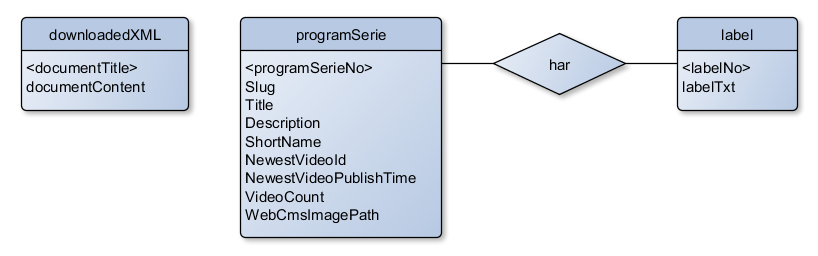
\includegraphics[width=1.1\textwidth]{pic/ER_programserie.png}
   \caption{ER-diagram over tabel-design.}
   \label{postgresql:ER-diagram}
\end{figure}

\section{Oprettelse af label�s}

N�r XML dokumentet er indl�st i tabellen downloadedXML, s� skal der som det f�rste oprettes labels til alle de kategorier, som findes i dokumentet programseries.xml. Til dette form�l er funktionen � getAndInsertAllLabels()�, som ses i figur \ref{ code: getAndInsertAllLabels} skabt. Denne funktion benytter et XPath-udtryk til at finde alle tekster til labels og for hver tekst den finder, s� unders�ges det om der allerede er oprettet en label med den tekst, hvis ikke s� inds�ttes denne nye label i tabellen. 

\begin{figure}[h]
\centering
\begin{BVerbatim}
  labels := (SELECT xpath('//ProgramSerie/Labels/string/text()', 
             downloadedXML.documentContent) FROM downloadedXML);
  FOR i IN array_lower(labels, 1) .. array_upper(labels, 1)
  LOOP
    SELECT labelNo INTO v_found FROM label WHERE label.labelTxt = labels[i];
    IF v_found IS NULL THEN
      INSERT INTO label(labelTxt) VALUES(labels[i]);
    END IF;
  END LOOP;
\end{BVerbatim}
\caption{Udsnit af funktionen getAndInsertAllLabels()}
\label{code: getAndInsertAllLabels }
\end{figure}

\section{Oprettelse af programserier samt label relationer}

For at identificere alle programserier, s� er funktionen �getAndInsertAllSlugs()� implementeret. Denne funktion finder med et XPath-udtryk alle programseriers \ele{slug} tag�s indhold og sender det videre til funktionen �getAndInsertSlugsDetail()�, som har til opgave et hente detaljerne ud og oprette relationer imellem programserierne og deres eventuelle label�s. Denne funktion ses i figur \ref{code:getAndInsertSlugsDetail}

\begin{figure}[h]
\centering
\begin{BVerbatim}
CREATE OR REPLACE FUNCTION getAndInsertSlugsDetail(p_slug VARCHAR) RETURNS VARCHAR AS $$
<< outerblock >>
DECLARE
  v_title                   text;
  v_description             text;
  v_shortName               text;
  v_newestVideoId           integer;
  v_newestVideoPublishTime  timestamp without time zone;
  v_videoCount              integer;
  v_webCmsImagePath         text;
  v_tag_value               text[];
  v_labels                  text[];
  v_programSerieNo          integer;
  v_labelNo                 integer;
BEGIN
  v_tag_value := (SELECT xpath('//ProgramSerie[Slug='''|| 
                  p_slug ||''']/Title/text()', 
                  downloadedXML.documentContent) FROM downloadedXML);
  v_title := v_tag_value[1];
  v_tag_value := (SELECT xpath('//ProgramSerie[Slug='''|| 
                  p_slug ||''']/Description/text()', 
                  downloadedXML.documentContent) FROM downloadedXML);
  v_description := v_tag_value[1];
  /**********************************************************/
  /* ...... samme metode for resten af variabelerne ....... */
  /**********************************************************/
  v_tag_value := (SELECT xpath('//ProgramSerie[Slug='''|| p_slug 
                  ||''']/WebCmsImagePath/text()', 
				  downloadedXML.documentContent) FROM downloadedXML);
  v_webCmsImagePath := v_tag_value[1];    
  INSERT INTO programSerie (Slug, Title, Description, ShortName, NewestVideoId, 
                            NewestVideoPublishTime, VideoCount, WebCmsImagePath)
  VALUES (p_slug, v_title, v_description, v_shortName, v_newestVideoId, 
          v_newestVideoPublishTime, v_videoCount, v_webCmsImagePath)
  RETURNING programSerie.programSerieNo INTO v_programSerieNo;

  v_labels := (SELECT xpath('//ProgramSerie[Slug='''|| p_slug 
               ||''']/Labels/string/text()', 
               downloadedXML.documentContent) FROM downloadedXML);
  IF array_lower(v_labels, 1) IS NOT NULL THEN
    FOR i IN array_lower(v_labels, 1) .. array_upper(v_labels, 1)
    LOOP
      SELECT labelNo INTO v_labelNo FROM label WHERE label.labelTxt = v_labels[i];
      IF v_labelNo IS NOT NULL THEN
        INSERT INTO slugLabel (programSerieNo, labelNo) 
		VALUES(v_programSerieNo, v_labelNo);
      END IF;
    END LOOP;
  END IF;
  RETURN v_title;
END;
$$ LANGUAGE plpgsql;
\end{BVerbatim}
\caption{Funktionen getAndInsertSlugsDetail()}
\label{code:getAndInsertSlugsDetail}
\end{figure}

\section{Funktionen til at finde programserier med specifik label}

Til videoapplikationen skal der som tidligere n�vnt bruges en funktion, som kan give et resultats�t af at programserier inden for en given kategori, alts� med en specifik label. Til det form�l er funktionen �programseriesOfLabel()� implementeret som tager kategori navnet som argument og er vist i figur \ref{code:programseriesOfLabel}. Den efterspurgte information er fordelt p� tre tabeller i PostgreSQL databasen og er: label, sluglabel og programserie.  
I denne funktion blev der anvend en cross join imellem de tre tabeller med efterf�lgende WHERE kondition for at finde alle programserie igennem deres programserieno som er registreret i tabellen sluglabel p� den efterspurgte label. Resultatet skal returneres XML formateret og skal kun vise nogle attributer af programserie. De inbygged PostgreSQL funktioner XMLRoot(), XMLAgg() og XMLElement() blev brugt og genererer en velformet XML dokument med r�deelement \ele{programseries} som indeholder de fundet elementer af \ele{programserie}. XML dokumentet mangler et DTD eller XML skema og den tilh�rende prolog for at blive en valid XML dokument.

\begin{figure}[h!]
\centering
\begin{lstlisting}[style=SQL]

CREATE FUNCTION programseriesOfLabel(labelName character(50) ) returns SETOF xml
AS $$
DECLARE

BEGIN
  
RETURN QUERY 
  SELECT XMLRoot(
    (SELECT XMLElement( name "programseries",
    XMLAgg( XMLElement( name "programserie",
        XMLElement( name "slug", ps.slug),
        XMLElement( name "titel", ps.title),
        XMLElement( name "description", ps.description),
        XMLElement( name "newestvideoid", ps.newestvideoid),
        XMLElement( name "newestvideopublishtime", ps.newestvideopublishtime)
        ) 
      )
    )
    
  FROM   programserie ps, sluglabel sla, label la
  WHERE  la.labeltxt = labelName
  AND    sla.labelno = la.labelno
  AND    sla.programserieno = ps.programserieno
  ), VERSION '1.0', STANDALONE yes
  );
  
END;
$$
LANGUAGE plpgsql;

\end{lstlisting}
\caption{Funktionen for at finde programserier registreret under en specifik kategori}
\label{code:programseriesOfLabel}
\end{figure}



\section{Funktionen til at finde programserier i et tidsinterval}

En yderlige funktion figur \ref{code:programseriesByPublishInterval} blev implementeret som g�r det muligt at s�ge efter programserier som blev offentligg�rd i et specifik tidsinterval. Ingen skal der returneres nogle attributer af de fundet programserier men denne gang sorteret med de nyste programserier f�rst. En ORDER BY kommando sorterer de fundet programserier med hensyn til attributet newestvideopublishtime inden de bliver udgivet pakket ind i XML. Den aggregationsfunktion XMLAgg() og den ORDER BY i kerne foresp�rgsel resulterer i en yderlige SELECT statement og dermed dybere nested SQL funktion. Med hj�lp af funktionen XMLRoot() returneres t velformet XML dokument. 


\begin{figure}[h!]
\centering
\begin{BVerbatim}
CREATE FUNCTION programseriesByPublishInterval(startTime timestamp, stopTime timestamp ) returns SETOF xml
AS $$
DECLARE

BEGIN
  RETURN QUERY SELECT XMLRoot(
  (SELECT XMLElement( name "programseries",
  XMLAgg( XMLElement( name "programserie",
        XMLElement( name "slug", sortedPS.slug),
        XMLElement( name "titel", sortedPS.title),
        XMLElement( name "description", sortedPS.description),
        XMLElement( name "newestvideoid", sortedPS.newestvideoid),
        XMLElement( name "newestvideopublishtime", sortedPS.newestvideopublishtime)
      )
  ))
  FROM 
  (
    SELECT *
    FROM programserie AS ps
    WHERE ps.newestvideopublishtime >= startTime AND  ps.newestvideopublishtime  <= stopTime
    ORDER BY ps.newestvideopublishtime DESC
  ) AS sortedPS), VERSION '1.0', STANDALONE yes); 
END;
$$
LANGUAGE plpgsql;

\end{BVerbatim}
\caption{Funktionen for at finde programserier i et specifik interval}
\label{code:programseriesByPublishInterval}
\end{figure}





\chapter{Konklusion}\label{chapter:conclusion}
I dette projekt kan det konkluderes at XML er et godt sprog til dataudveksling, hvor enkelte objekter, fx i form af detaljer omkring en video eller en programserie skal udveksles. Is�r ses XML sproget som v�rende godt til online verdenen, hvor der ligefrem l�gger op til at outputtet data direkte som HTML. 

XML kommer derimod i problemer n�r der er tale om at holde p� mange informationer med tilh�rende relationer. Her t�nkes fx p� problemstillingen omkring alle programserier i et dokument, og alle informationer omkring de tilh�rende videoer i et andet dokument. Dokumenterne kan uden problemer, indeholde alt informationen, men der findes igen metode ti l at sikre at relationerne imellem de to dokumenter rent faktisk er eksisterende. En video i XML dokumentet med detaljer om videoerne kan godt referere til en programserie i XML dokumentet omkring alle programserierne, men der er ikke nogen sikkerhed for programserien rent faktisk findes i dette dokument. Her savnes princippet med fremmen�gler fra den relationelle database. Til gengl�de er XML et meget l�sebart sprog for det menneskelige �je, hvor der kan hurtigt skabes et overblik over dataenes hierarkiske struktur, hvilket kan v�re meget vanskeligt n�r der ses p� tabeller i en relationel database.

Omkring XQuery, s� konkluders det at syntaksen er noget speciel og uvant i forhold til andre sprog. Specielt blev det bem�rket, at det ikke kan lade sig g�re at skrive en IF-s�tning uden, at der skal med tages en ELSE, da denne er p�kr�vet ogs� selvom den ikke skal have noget indhold.    

XML skema.( skal altid ske ved indl�sning) Dermed undg�es fejl (som dynamisk fejl) n�r data type �ndres.

Funktioner til oversigt og med specfik detajler til valg af video.



\newpage
\clearpage \thispagestyle{empty}
\begin{appendix}
\chapter{Installations guide}
\subsection{Fil beskrivelse}


\subsubsection{XML data dokuments}

\begin{itemize}
\item \textbf{all.xml} Video (�ldre version) Indholder detaljeret information om alle videoer.
\item \textbf{all\_new.xml} Video (nyere version)
\item \textbf{programseries.xml} Programserie (�ldre version) med informationer om alle tilg�ngelige serier.
\item \textbf{programseries\_new.xml} Programserie (nyere version)
\end{itemize}



\subsubsection{XML Skemaer}

\begin{itemize}
\item \textbf{all\_schema.xsd} Skema til all\_x.xml filer
\item \textbf{programseries\_schema.xsd} Skema til programseries\_x.xml filer
\end{itemize}


\subsubsection{XQuery og XPath foresp�rgsler}

\begin{itemize}
\item \textbf{dr\_api\_module.xqm} XQuery modul med de fleste foresp�rgsler
\item \textbf{dr\_api\_module\_usage.xq} Eksempel som viser hvordan modulet dr\_api\_module.xqm bruges.
\item \textbf{word\_cloud\_search.xq} Foresp�rgsel til ord sky funktionen.
\item \textbf{text\_search-Restaurant-laks.xq} Full-text s�gning i programserie.
\item \textbf{ful-text-search-SCORE-Restaurant-laks.xq} Full-text s�gning i programserie med score information.

\end{itemize}


\subsubsection{Supplerende filer}

\begin{itemize}
\item{stop-words.txt} List med brugte stop ord til full-text s�gning.
\end{itemize}



\subsection{BaseX konfiguration}
I projektet blev brugt BaseX 7.8.1.

Opret en ny database i BaseX med \textit{Database - New} kommando for hver af filerne, programseries.xml, programseries\_new.xml, all.xml og all\_new.xml. Det er vigtigt at v�lge \textit{Indexes} i menuen \textit{Create Database}, hvis Full-Text index skal aktiveres. Sprog s�ttes til dansk og stop-word.txt filen bliver valgt som vist p� figur \ref{inst:BaseXIndex}.

\begin{figure}[h!]
  \centering
   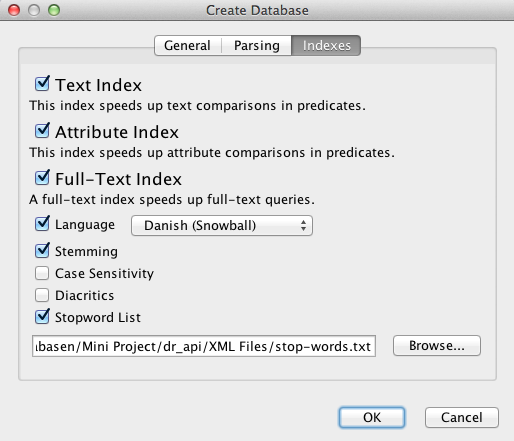
\includegraphics[width=0.8\textwidth]{pic/BaseX-Index.png}
   \caption{BaseX - Full-Text index indstilling }
	\label{inst:BaseXIndex}
\end{figure}


\subsection{PostgreSQL konfiguration}

\begin{enumerate}

    \item Opret en ny database, eksempelvis: dr\_api
	\begin{verbatim}
	CREATE DATABASE dr_api;
	\end{verbatim}

	\item K�r skriptet som opretter alle tabeller.
	\begin{verbatim}
	create_tables.sql
	\end{verbatim}

	\item K�r skriptet for at kopierer XML indhold ind i databasen.
	\begin{verbatim}
	insert-XMLinto-downloadedXML.sql
	\end{verbatim}	

	\item K�r skriptet for at installere alle funktioner.
	\begin{verbatim}
	functions.sql
	\end{verbatim}	

	\item K�r skriptet for at opdatere de forskellige tabeller.
	\begin{verbatim}
	CREATE_ALL_DATA.sql
	\end{verbatim}	


\end{enumerate}




\end{appendix}

\end{document} 